\begin{frame}{Formalities}
\begin{center}
\begin{tabular}{rl}
Email: & agilesteel@gmail.com\\
Credits: & 3\\
Exam: & K 60 - 90\\
Room: & F 0.35\\
Time span: & 12:15 - 13:45\\
Slides: &
\link{http://85.214.74.39/lectures/scala}{http://85.214.74.39/lectures/scala}
\end{tabular}
\end{center}
\end{frame}
\begin{frame}{What is this course about?}
\begin{description}
\item[80\%] Programming in Scala
\begin{itemize}
	\item Syntax
	\item Semantics
\end{itemize}
\pause
\item[20\%] Software development
\begin{itemize}
 	\item Programming languages
 	\item Programming disciplines
\end{itemize}
\end{description}
\end{frame}
\begin{frame}{What is the goal of this course?}
\begin{center}
The goal is to give a head start on learning Scala.
\pause
\begin{figure}[ht]
	\centering
  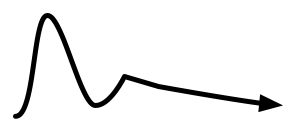
\includegraphics{resources/ScalaComplexity.png}
	\\Scala's learning curve
\end{figure}
\end{center}
\end{frame}